\documentclass{article} % For LaTeX2e
% We will use NIPS submission format
\usepackage{nips13submit_e,times}
% for hyperlinks
\usepackage{hyperref}
\usepackage{url}
% For figures
\usepackage{graphicx} 
\usepackage{subfigure} 
% math packages
\usepackage{amsmath}
\usepackage{amsfonts}
\usepackage{amsopn}
\usepackage{ifthen}
\usepackage{natbib}

\title{Project-I by Group OSLO}

\author{
Etienne Pot\\
EPFL \\
\texttt{etienne.pot@epfl.ch} \\ \And 
Lucile Madoulaud\\
EPFL \\
\texttt{lucile.madoulaud@epfl.ch} \\
}

% The \author macro works with any number of authors. There are two commands
% used to separate the names and addresses of multiple authors: \And and \AND.
%
% Using \And between authors leaves it to \LaTeX{} to determine where to break
% the lines. Using \AND forces a linebreak at that point. So, if \LaTeX{}
% puts 3 of 4 authors names on the first line, and the last on the second
% line, try using \AND instead of \And before the third author name.

\nipsfinalcopy 

\begin{document}

\maketitle

\begin{abstract}
This report present our method and prediction results of for the regression and classification tasks. For the regression task, we have decided to train three different models and a model selector, we obtain respectable performance except for some outliers which have too much impact on our RMSE. We discuss about some improvement possible to solve this problem.\newline
For the classification task, we have decided to train two different models this time, but here the results are less good, we discuss about some possibilities to improve them.
\end{abstract}

\section{Data Description}
Our training data $\mathbf{X}$ which consists in $N=2800$ data of 65 variables for the regression and $N=1500$ data of 29 variables for the classification task. Our testing set is composed of $1200$ and $1500$ sample for the regression and classification.
\newline
Our goal is to produce predictions for the test sample, as well as an approximation of the test-error.

\section{Data visualization and cleaning}
First of all, we have done some exploration of our data before we start to apply some machine learning algorithms.

\subsection{Regression}

On the regression task, by plotting the histogram of the output (Figure \ref{fig:histY}), we can clearly see three distinct clusters around 2000, 6000 and 12000.

We have also plotted each variable in function of the output to see if there was some variable directly correlated to our output. We have see for instance that the variables 16 and 38 could help us to discriminate between the three clusters (Figure \ref{fig:clusters}) and that for each cluster, there was a variable which was strongly linearly correlated with the output (12, 26 and 61), those could eventually be used to have a first really simple model with only one dimension.

\begin{figure}[!h]
\center
\subfigure[Histogram of $\mathbf{y}$. We clearly see three clusters.]{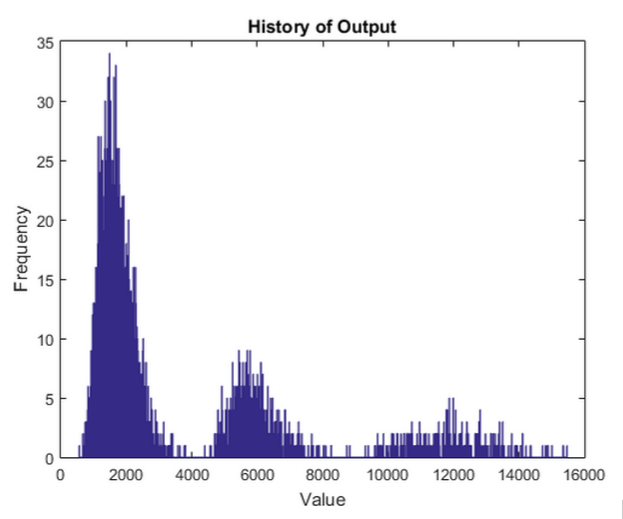
\includegraphics[width=2.5in]{figures/histY.png} \label{fig:histY}}
\hfill
\subfigure[Output in function of two interesting variables. We have separated our output in three different clusters]{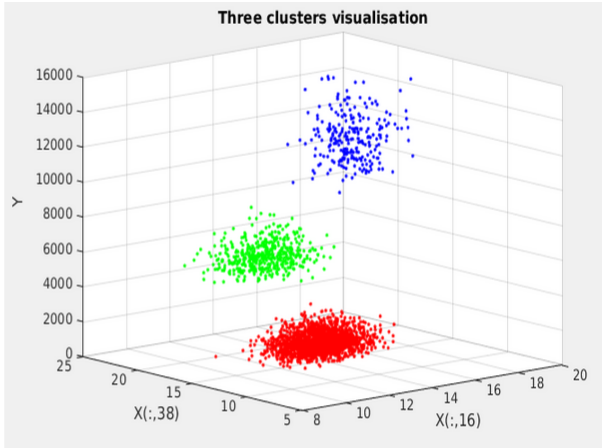
\includegraphics[width=2.5in]{figures/clusters.png} \label{fig:clusters}}
\caption{}
\end{figure}

\subsection{Classification}

Similarly, for the classification task, by plotting the histogram of the $\mathbf{X}$ (for instance column 10), we see that our input seems to be the sum of two Gaussian distributions. We have also used those histogram to isolate and remove some outliers which were really far from the Gaussian distributions.

We have also notice that when we separate the two Gaussian distributions, some variables where strongly correlated with the output class, we have also visualized the combination of two variables using gplotmatrix to see if we could see some pattern between the variables, we didn't.

\begin{figure}[!h]
\center
{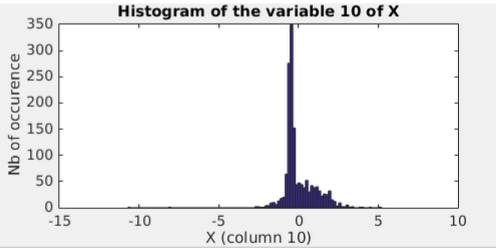
\includegraphics{figures/histX10.png} \label{fig:histX10}}
\caption{Histogram of variable 10 of $\mathbf{X}$. We see the two gaussian and some outliers.}
\end{figure}

We also remark that our training set possess more sample of class +1 than class -1 (65\% vs 35\%).

\section{Regression models}
At first, we have try to train all our data with a single model. It was not going well (huge RMSE) so we have decided to separate our data into three different model for the regression task corresponding to the three clusters we have seen in our training data. In order to do that, we will also need to another model which will choose which one of the three model apply to the testing data.

To avoid bias, we have separated our training set in two parts (90\%-10\%): the first one to train (and test using cross validation) the three (regression) / two (classification) models, and the other one to test the model selection and estimate the global error.

Our input matrix being ill-conditioned, we have decided to focus on using ridge regression which will lift the eigenvalue to avoid the problem. And selecting the best value of lambda for each of our model.

We have separated the first part of our training values (the 90\%) into three groups corresponding to the output clusters. We have then trained and tested each model independently.

After feature transformation, we have obtain the following results presented in Figure \ref{fig:learningCurves}.

\begin{figure}[!h]
\center
{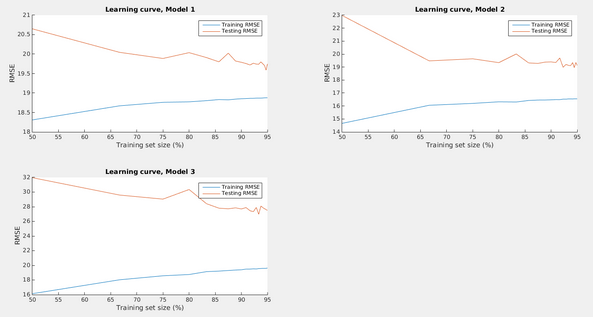
\includegraphics{figures/learningCurves.png} \label{fig:learningCurves}}
\caption{Histogram of variable 10 of $\mathbf{X}$. Learning curves for each of our models}
\end{figure}

Here are our three model results on the testing set for a 15-cross validation:
\begin{enumerate}  
        \item Model 1:  rmse = 19.6      ; std = 1.8
        \item Model 2:  rmse = 19.0      ; std = 3.1
        \item Model 3:  rmse = 27.4      ; std = 5.8
\end{enumerate}

Each cluster size being large from about 4000, having a rmse of about 15-30, is not perfect but is still ok to have a good estimation of y. Our model 3 has the worst results, and a higher variance, our model 1 provide the best results and has the smaller variance. Luckily, there is much more points in our model 1 which perform the best and few in the one which perform the worst.

\section{Classification models}

Similarly, for the classification task,  we have separated our training data into two parts corresponding to the two Gaussians distribution. We have done that by using the column 12 where the Gaussian distributions were already separated, and we have then checked that the data where also separated for the other columns.

For our classification models, after having try without success to solve our ill-conditioning input matrix by reducing the dimension we conclude we had to use the penalized logistic regression. In order to have the better results possible, we needed a small alpha with a great number of iteration, which made the convergence really slow (in addition we also needed to compute the best lambda using cross-validation, which made the program even slower).

To improve the convergence speed, as well as the global performances, we also have try to apply Iterative Recursive Least-Squares, but the ill-conditioning made our beta diverge to infinity. After few try, we have stopped using this method and went back to penalized logistic regression.

The results predicted with our model were not good (30-45\% of mistake on the global error). A lack of times prevent us to do some diagnostic to identify were was the problem with our results. Our model had a bias toward the -1 class. Even if this class was minority into our training set, our model predict more -1 than +1.

\section{Feature transformation}

We have tested different features transformations to see if those could improve our results.

First for the categorical data, on both regression and classification model, we have try dummy encoding, keeping only the binary data or removing all. Each test has few impact on our results (even slightly worse in case of dummy encoding) so we have decided to remove the categorical data.

We also have try data reduction by removing the features which had the strongest negative impact on our RMSE. In order to do that, we have created a script which remove one of the input column and record the result, we have repeated the process 200 times for each column to see if there was significant differences. The results were not concluding so we have stopped the experimentation here.

Finally, we have tested simple and usual global features transformations apply to all input column. Here are the transformation we have tested: , $x^2$, $x^3$, $x^4$, $exp(x)$, $1/x$, $sqrt(x)$, $log(x)$, $abs(x)$.

For the regression task, we remarked that $x^2$ and in a higher degree $x^3$ had a big impact on the results (RMSE divided by a factor 2-4 for each of our model).

We did not have the time to test all those transformation on the classification task.

\section{Model selection}

\subsection{Regression}

At first, to decide which model to apply to our points, we have apply a naive threshold separation method (on the columns 16 and 38). It was not going very well because the “borderlines” point where easily confused with the wrong model.

This part is critical because even if few points are incorrectly predicted with the wrong model, the error is to huge and it has a really big impact on the rmse.

In order to improve the result of the model selection, we have try KNN. It was simple enough to implement and has greatly improved our results. From our different tests, 3-NN seems the one which produced the better results (2-3\% of wrong classification).

When we evaluate the global error (including the model selection), we remark that most points are correctly predicted except for those few points which are incorrectly classified (fig.\ref{fig:predErrors}), because we apply the wrong model to predict them. One way to solve this issue could have been to change the cost function (by using for instance the tukey biweight loss). The errors would still be there but will be less penalized. Of course it’s depend of our application and if it’s okay to have those kind of mistake.

\begin{figure}[!h]
\center
{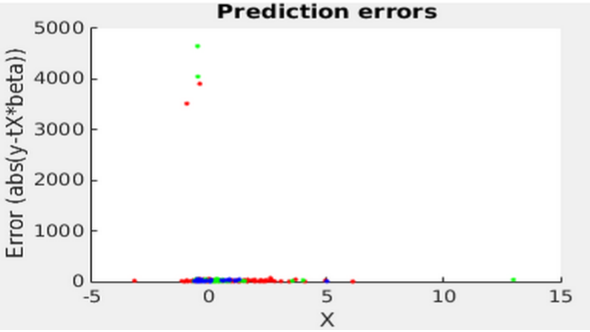
\includegraphics{figures/predErrors.png} \label{fig:predErrors}}
\caption{For our regression model: all our predicted points have a low error value except for the four points which have been wrongly classified}
\end{figure}

With this model, we can also estimate the confidence of the prediction for each point. Indeed, for most of the points, we are confident to use the right model (all neighbours belongs to the same class), and if we remove the few points for which we are not sure (have neighbour in two different classes), it drastically improve our results (RMSE goes from 600-800 to 21 by removing the 6\% of our points for which we are not sure which model to apply).

In order to correct those outliers, we have tried to apply a basic outlier detection by looking at the distance of each points to the mean of his cluster and see if some points where outside this Gaussian distribution. Unfortunately, even outliers point where not distant enough of the mean to allowing us to detect them. We did not have enough time to try more complex method, though it would have been necessary.

\subsection{Classification}

Separate the models on the testing set was easier on the classification task because it was not dependant of the output, so we separate the testing set the same way that the training set, by putting a threshold on the variable 12 of our input vector. We have checked that we obtain the same distribution for the testing set that for our training set.

\section{Final prediction}

\subsection{Regression}

For the final prediction, we have retrain our data set on all the given data. Even if we could not check if our prediction are correct or not, we can compare the histogram of our predicted values (fig. \ref{fig:histPredY}) with the histogram of the output value of our training set (fig.\ref{fig:histY}). Those two were similar. We also have checked that the proportion of data in each cluster was similar to the one in our training set (70\% for cluster 1, 20\% for cluster 2 and 10\% for cluster 3).

\begin{figure}[!h]
\center
{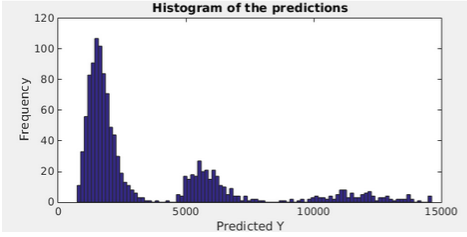
\includegraphics{figures/histPredY.png} \label{fig:histPredY}}
\caption{The distribution of our predicted Y on the testing set is really similar to the one given on the training set (fig \ref{fig:histY})}
\end{figure}

With those informations, we can suppose that the testing predictions will be quite similar to the one given with our training set. Unfortunately, that also means that some point will be incorrectly classified (about 36 of 1200 points, we can even know which one are potentially wrong), we also know that it will have a strong negative impact on our final RMSE. After running several times our algorithm, we predict the final error: 630 +/- 200 . The high variance of the prediction is due to the fact that our model is really sensitive to outliers so just one more or one less outlier can have a big impact on our rmse.

\begin{figure}[!h]
\center
{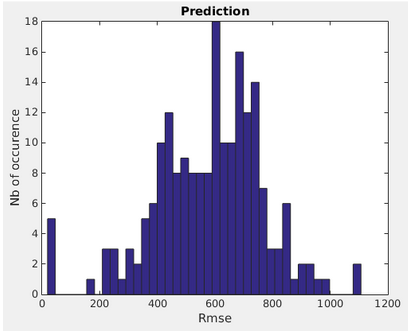
\includegraphics{figures/histPred.png} \label{fig:histPred}}
\caption{After running 200 times our algorithm, we can have a pretty good estimation of our rmse. (fig \ref{fig:histPred})}
\end{figure}

\subsection{Classification}

Even after having separated the data into two model and apply the predictions on each model individually, the results seems still pretty random. By applying the same method that above on the optimal computed lambda for each of the models, we predict an error of 40\% +/- 10\%.

\section{Conclusion}
\subsection{Regression}
We could have spend more time focusing on improving each one of the three model performances (for selecting the best parameters) but we have decided instead to focus more on the model selection part, indeed, the three models performances was already quite good and the main problem with our final results is that the few outliers points ruin all our performances.

\subsection{Classification}
An unidentified problem make the results of our classification not good. In addition, the penalised logistic regression was really slow, which create a big delay for each test before we could have a feedback. For this reason among other, we have tested much less configurations for the classification that for the regression. And in conclusion, we did not find any satisfying model for the classification task.

\subsubsection*{Acknowledgments}
All the code and the report was written by us, except for the small parts provided during the lab sessions (for instance, some part of the code for the IRLS came from the lecture slide on logistic regression (p8)).

\end{document}
